% !TeX root = ../thuthesis-example.tex

\chapter{补充内容}
\label{appendix}
\section{插图}
以下为在FFHQ数据集上测试的结果展示
\begin{figure}[H]
  \centering
  \begin{minipage}[b]{0.3\linewidth}
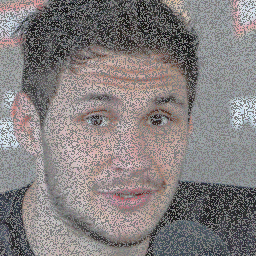
\includegraphics[width=\linewidth]{Picture/input/00004.png}
    \caption{加噪图像4}
    \label{noised image }
  \end{minipage}
  \hspace{0.1cm} % Space between images
   \begin{minipage}[b]{0.3\linewidth}
    
\includegraphics[width=\linewidth]{Picture/label/00004.png}
    \caption{原始图像4}
    \label{original image }
  \end{minipage}
\hspace{0.1cm}
  \begin{minipage}[b]{0.3\linewidth}
    
\includegraphics[width=\linewidth]{Picture/recon/00004.png}
    \caption{还原图像4}
    \label{inpainted image}
  \end{minipage}
\end{figure}



\begin{figure}[H]
  \centering
  \begin{minipage}[b]{0.3\linewidth}

\includegraphics[width=\linewidth]{Picture/input/00005.png}
    \caption{加噪图像5}
    \label{noised image }
  \end{minipage}
  \hspace{0.1cm} % Space between images
   \begin{minipage}[b]{0.3\linewidth}
    
\includegraphics[width=\linewidth]{Picture/label/00005.png}
    \caption{原始图像5}
    \label{original image }
  \end{minipage}
\hspace{0.1cm}
  \begin{minipage}[b]{0.3\linewidth}
    
\includegraphics[width=\linewidth]{Picture/recon/00005.png}
    \caption{还原图像5}
    \label{inpainted image}
  \end{minipage}
\end{figure}

\begin{figure}[H]
  \centering
  \begin{minipage}[b]{0.3\linewidth}
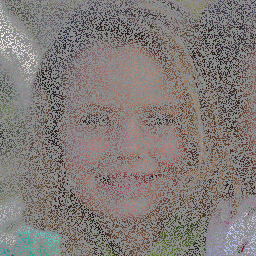
\includegraphics[width=\linewidth]{Picture/input/00006.png}
    \caption{加噪图像6}
    \label{noised image }
  \end{minipage}
  \hspace{0.1cm} % Space between images
   \begin{minipage}[b]{0.3\linewidth}
    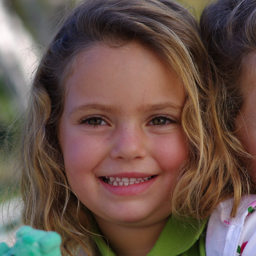
\includegraphics[width=\linewidth]{Picture/label/00006.png}
    \caption{原始图像6}
    \label{original image }
  \end{minipage}
\hspace{0.1cm}
  \begin{minipage}[b]{0.3\linewidth}
    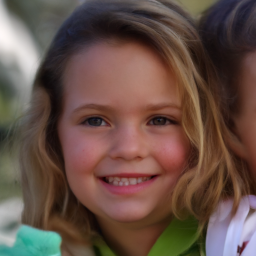
\includegraphics[width=\linewidth]{Picture/recon/00006.png}
    \caption{还原图像6}
    \label{inpainted image}
  \end{minipage}
\end{figure}


\section{实验说明}
本项目为开源项目,可以直接从github上获取本项目代码,在终端输入如下命令行。1. 拷贝项目
\label{experiment instructions}
\begin{lstlisting}[language=bash]
git clone git@github.com:JamesJunyuGuo/Graduation_Project.git
cd Graduation_Project/
\end{lstlisting}
2. 下载预训练集。 参考github仓库\href{https://github.com/openai/guided-diffusion.git}{https://github.com/openai/guided-diffusion.git}可以点击进入网页下载对应的预训练集。在主文件夹中新建一个新文件夹 models/ 并将下载的预训练集放到里面。
\begin{lstlisting}[language=bash]
mkdir models
mv {DOWNLOAD_DIR}/ffqh_10m.pt ./models/
mv {DOWNLOAD_DIR}/lsun_bedroom.pt ./models/
\end{lstlisting}
3. 本地环境配置
\begin{lstlisting}[language=bash]
conda create --name DM python=3.8

conda activate DM

pip install -r requirements.txt

pip install torch==2.2.2
\end{lstlisting}
4. 训练过程   
执行训练只需要在本地命令行输入如下代码
\begin{lstlisting}[language=bash]
python3 sample_test.py \
--model_config=configs/LSUN_config.yaml \
--diffusion_config=configs/diffusion_config.yaml \
--task_config=inpainting_config.yaml;
\end{lstlisting}
其中可以根据具体的下游任务类型修改yaml文件中的具体配置,例如在任务设置参数中可以修改root以及name更改读取数据集位置以为选取不同的下游任务进行训练,文件配置内容如下可见。
\begin{lstlisting}[language=bash]
conditioning:
    method: ddim 
    params:
        scale: 1.0

data:
    name: LSUN
    root: ./data/samples/

measurement:
    operator: 
        name: inpainting # check candidates in guided_diffusion/measurements.py

noise:
    name:  gaussian 
    sigma:  0.05 
\end{lstlisting}






